
%%******************************************************************************
%% SECTION - Materials 

%%******************************************************************************



\section{Sonar}
\label{sonar}


\begin{table}[ht!]

	\begin{tabular}{r l|l p{12cm} }
		
		\textcolor{gray}{Especificação} &&& 	{Profiler Super Seaking DFP}\\
		\textcolor{gray}{Data} &&& 				{26/03/2014}\\
        \textcolor{gray}{Beneficiado} &&&		{Tritech} \\
        \textcolor{gray}{CNPJ} &&& 				{Internacional} \\
        \textcolor{gray}{Número Nota} &&& 		{Pendente a entrega do equipamento} \\
		\textcolor{gray}{Quantidade} &&& 		{1} \\
		\textcolor{gray}{Valor} &&& 			{R\$41.904,16} \\
		\textcolor{gray}{Data Sheet} &&& 		{Anexo I - \ref{seaking_profiler}} \\
		\textcolor{gray}{Código de Rastreamento} &&& {61014} \\

		\textcolor{gray}{Função no projeto} &&& {O Sonar será utilizado para realizar o mapeamento 3D do trilho do Stoplog. O mapeamento permite que o operador observe se existe ou não detritos no trilho que impossibilitariam o posicionamento correto do Stoplog para a vedação. } \\
		\textcolor{gray}{Razão da Escolha} &&& {Dentre os sonares analisados que possuem a especificação necessária para o projeto o Profiler Super Seaking da Tritech apresentou o menor custo.   
		 \begin{itemize}
		  \item \textbf {Super Seaking da Tritech por R\$41.904,16}
		  \item BV5000 da Blueview por \$ 138.000,00 
		  \item DT-101 da Imagenex por R\$ 365.000,00
		\end{itemize}}

	\end{tabular}
\end{table}

\newpage

\subsection{Foto do Material}
\begin{figure}[H]
 \centering
 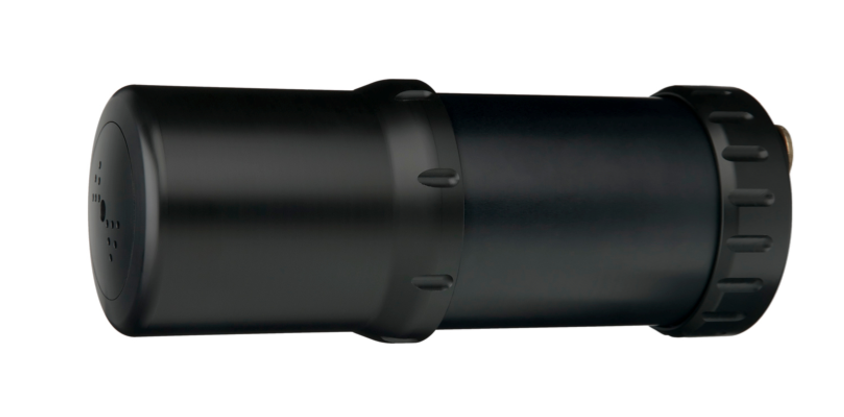
\includegraphics[width=1\columnwidth]{Seaking_Profiler/foto.pdf}
 \caption{Profiler Super Seaking}
\end{figure}

\subsection{Cotação Sonar 1 }
\begin{figure}[H]
 \centering
 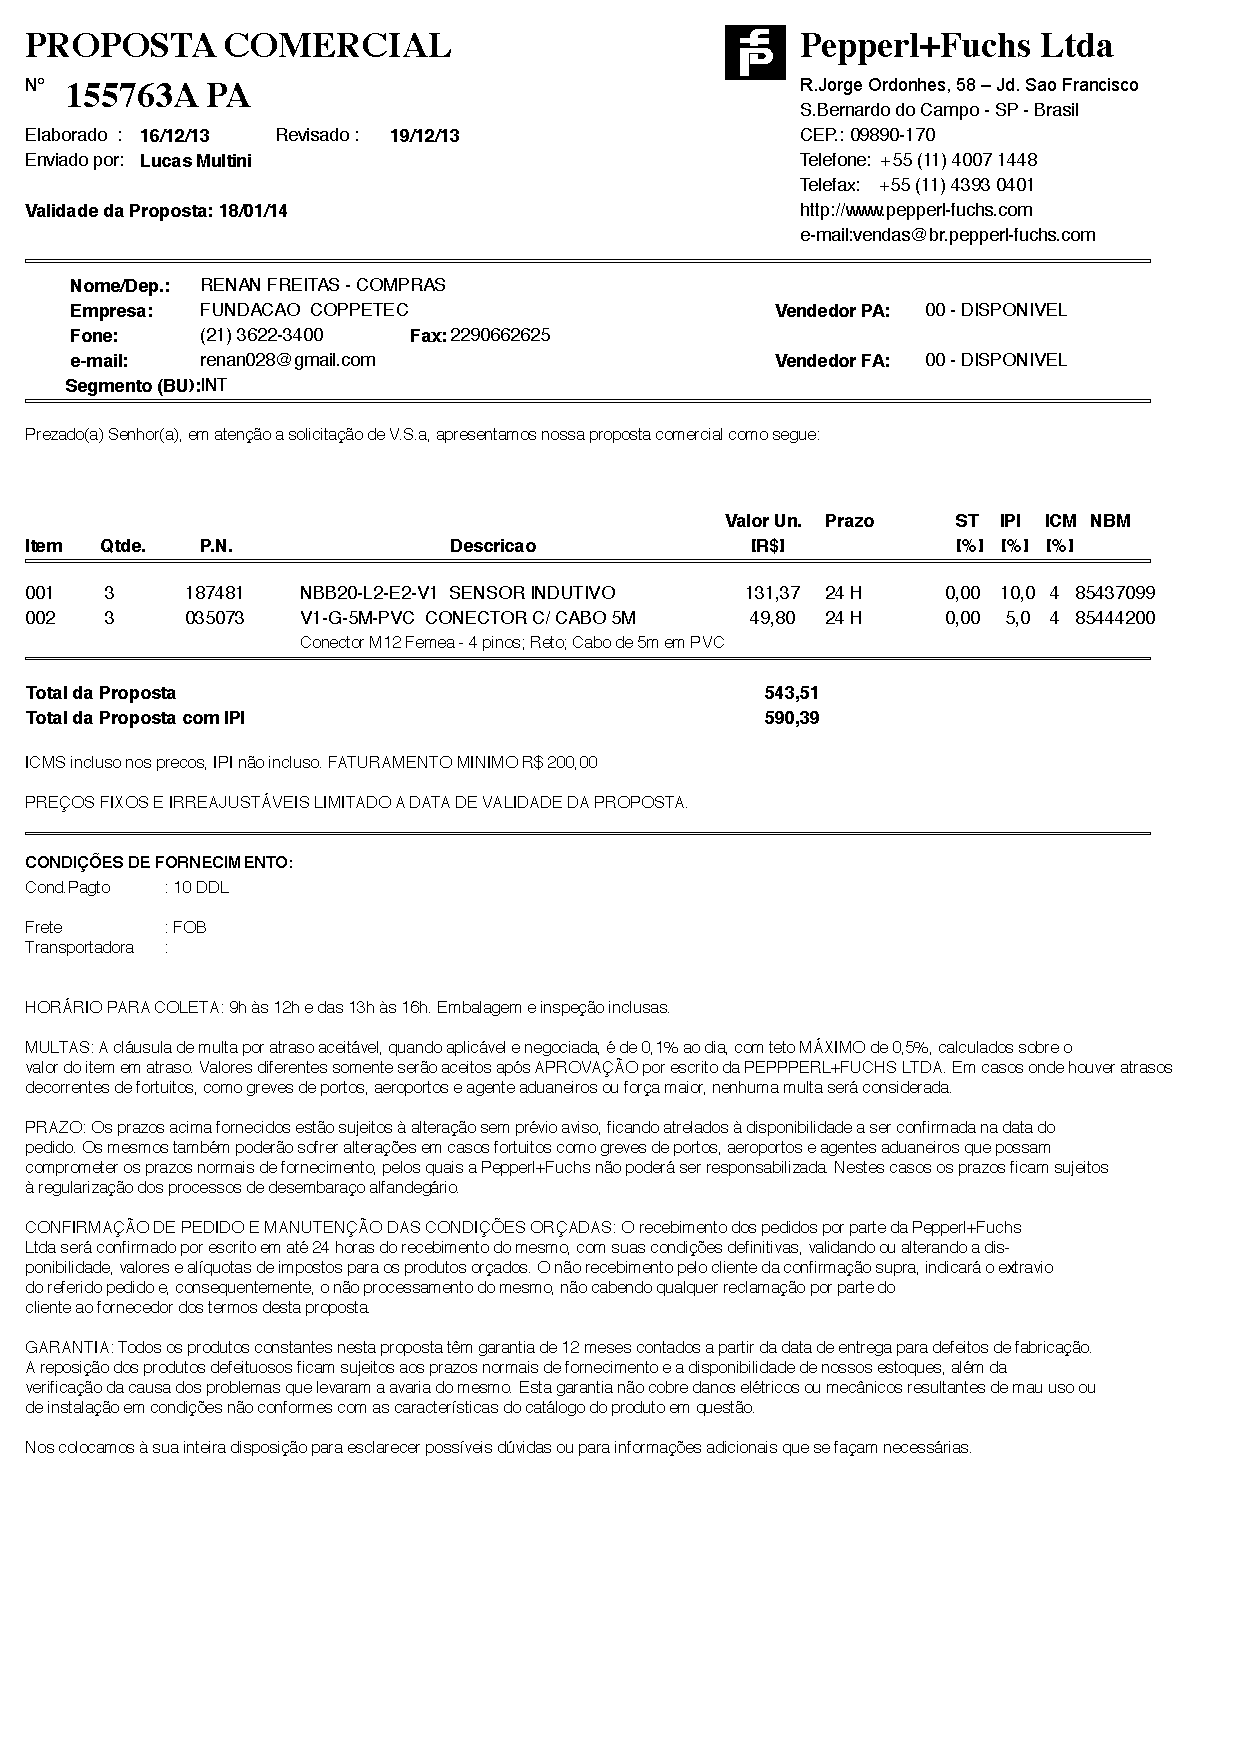
\includegraphics[width=1\columnwidth]{Seaking_profiler/price_quote_0.pdf}
 \caption{Cotação Super Seaking DFP da Tritech}
\end{figure}

\subsection{Cotação Sonar 2 }
\begin{figure}[H]
 \centering
 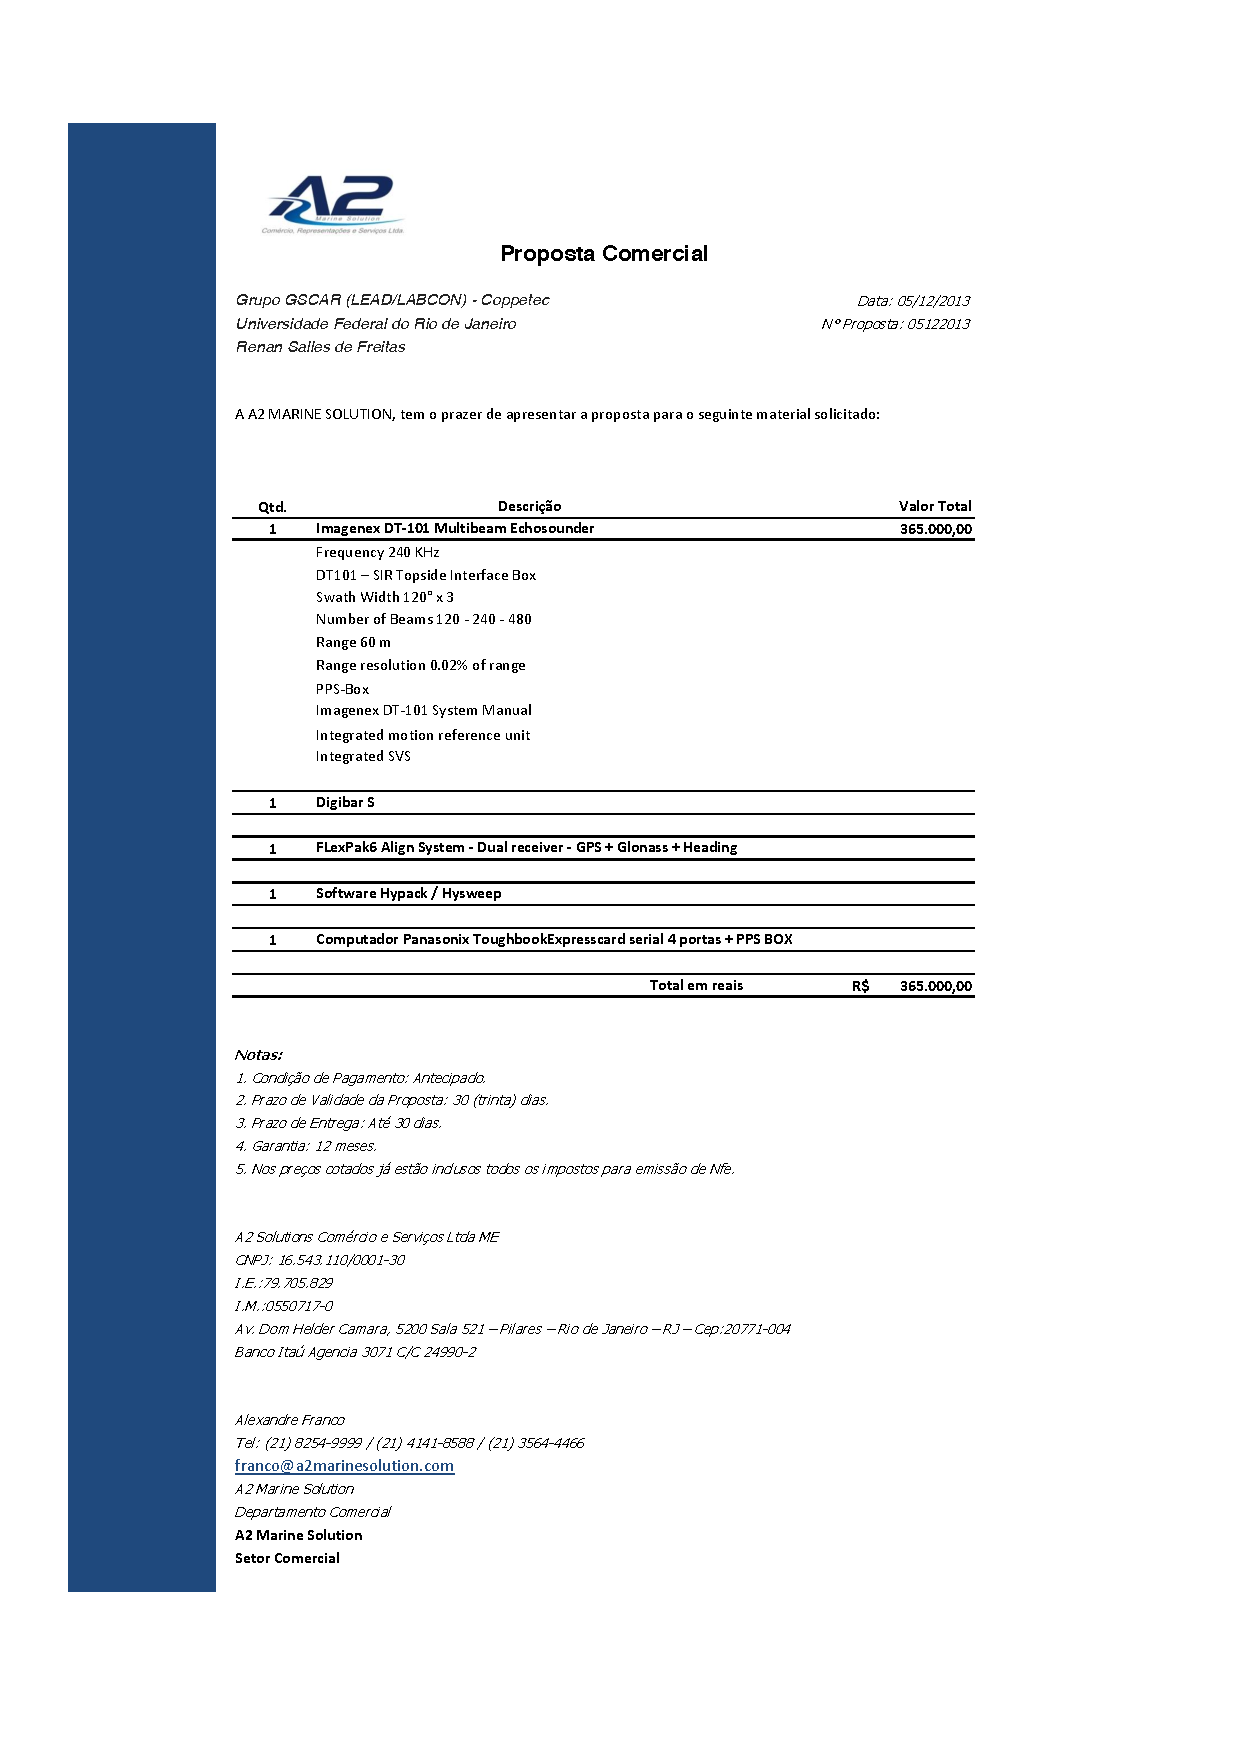
\includegraphics[width=0.9\columnwidth]{Seaking_profiler/price_quote_1.pdf}
 \caption{Cotação DT-101 da Imagenex}
\end{figure}

\subsection{Cotação Sonar 3 }
\begin{figure}[H]
 \centering
 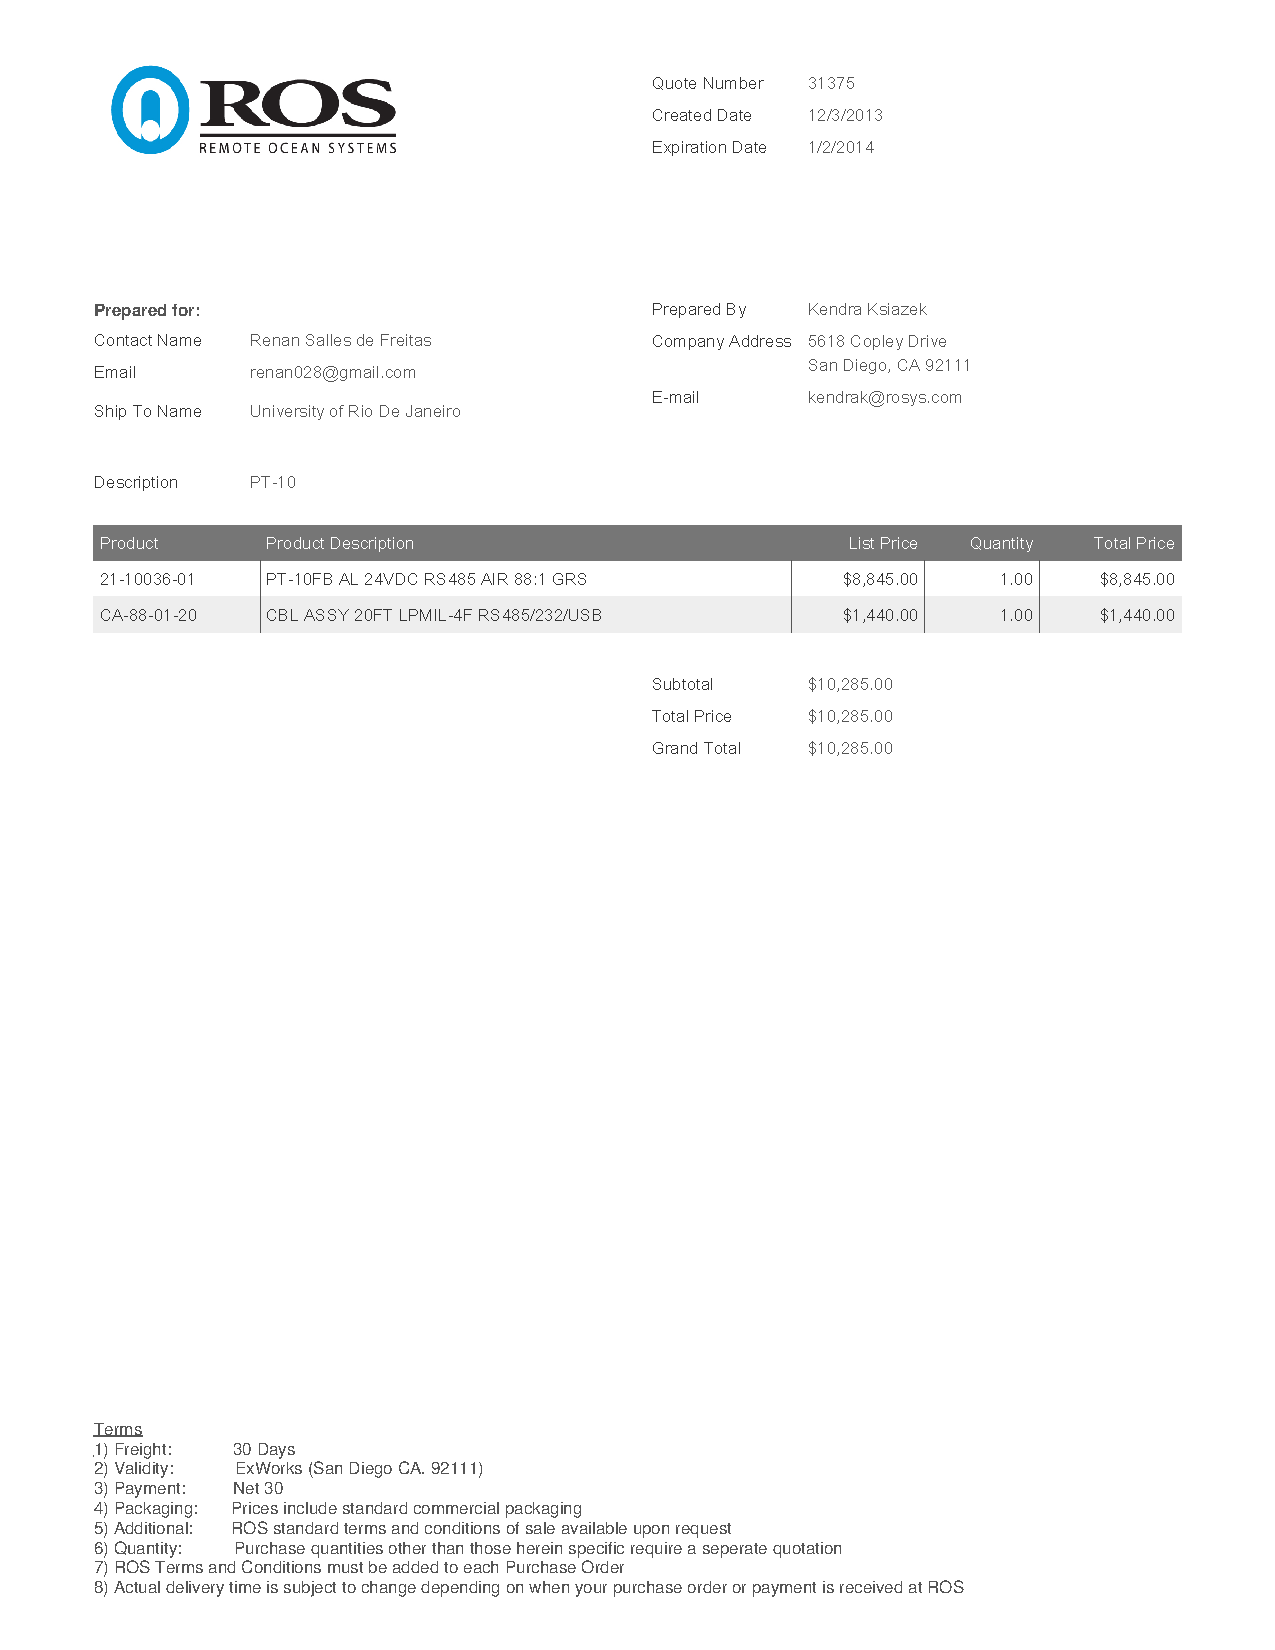
\includegraphics[width=1\columnwidth]{Seaking_profiler/price_quote_2.pdf}
 \caption{Cotação BV5000 da Blueview}
\end{figure}

\subsection{Nota Fiscal}
\begin{figure}[H]
 \centering
 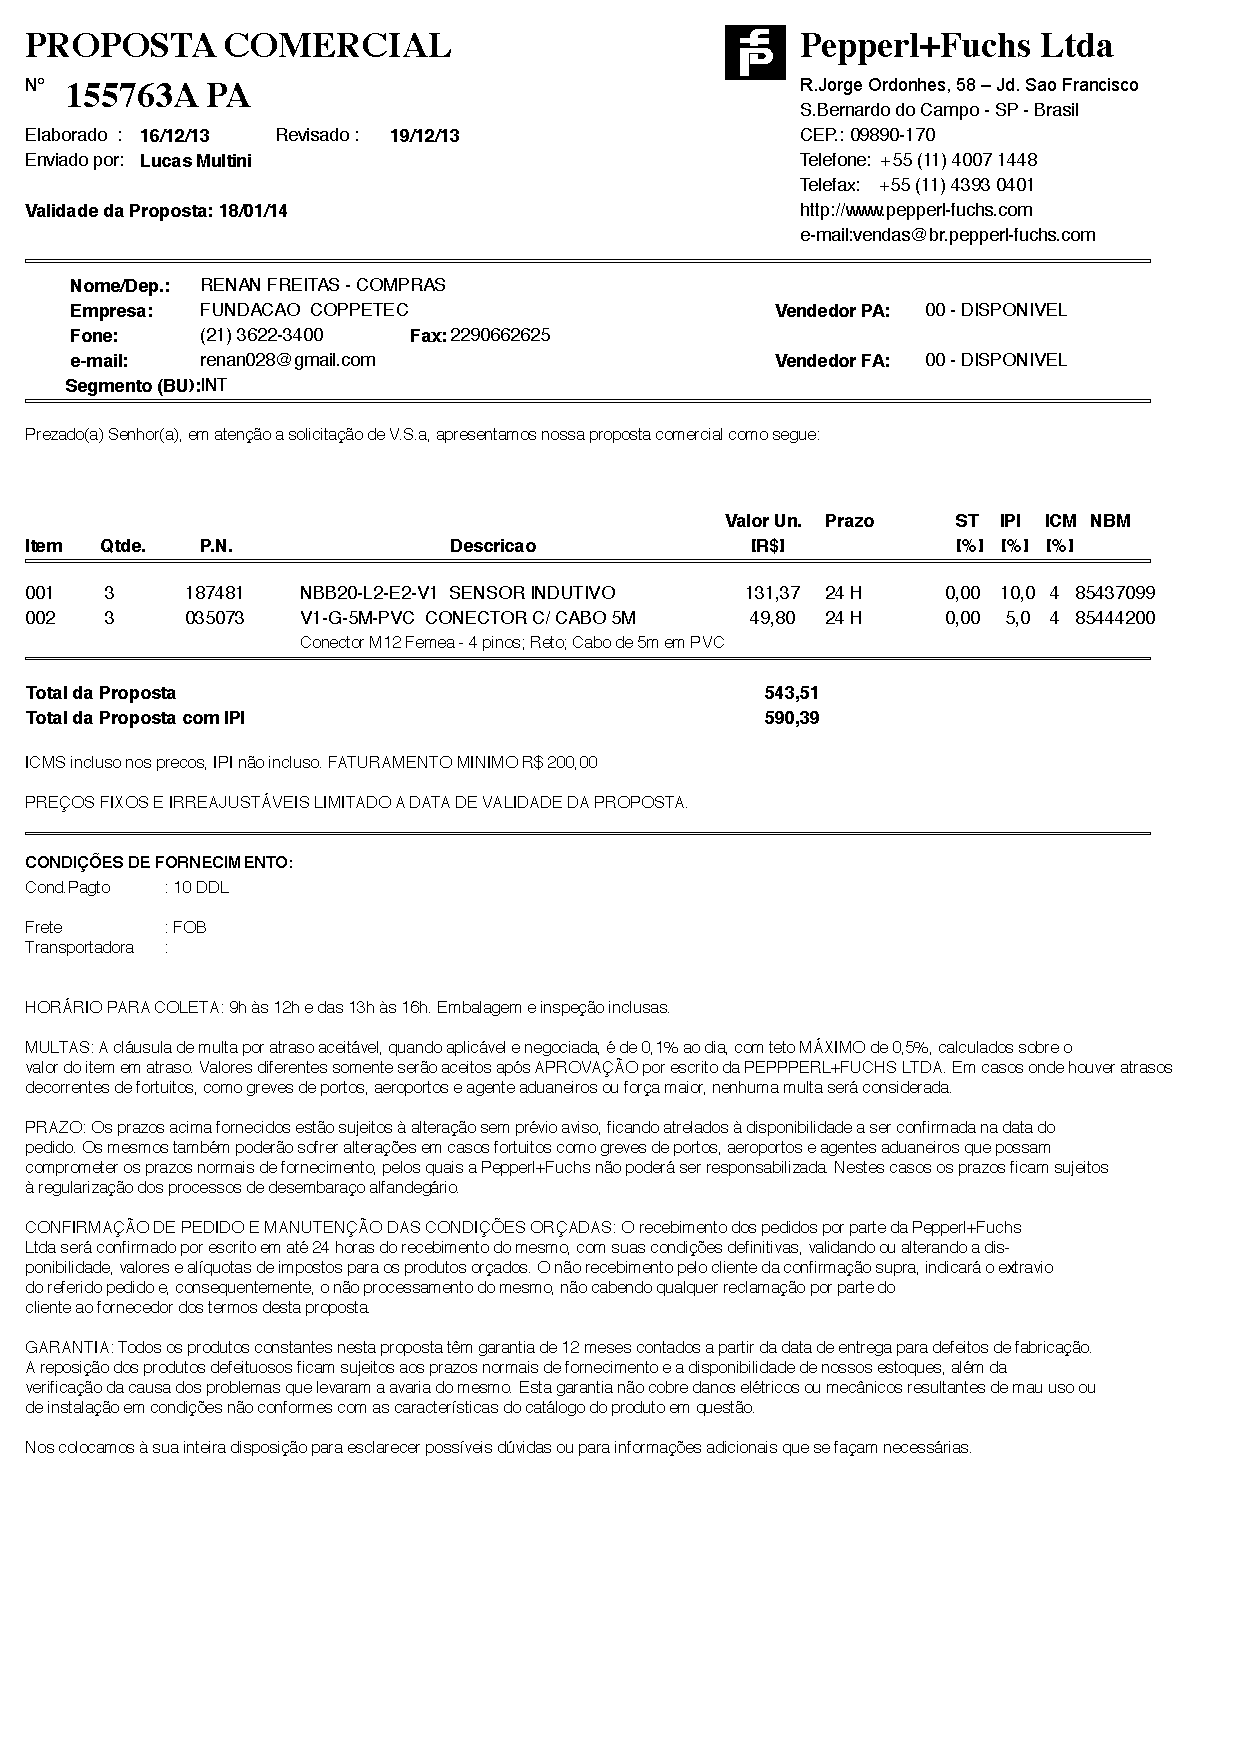
\includegraphics[width=1\columnwidth]{Seaking_profiler/price_quote_0.pdf}
 \caption{Nota fiscal do Sonar Super Seaking DFP da Tritech}
\end{figure}


